\documentclass[11pt,letterpaper]{article}
\usepackage[margin=2cm,includefoot]{geometry}
\usepackage[spanish]{babel}

\usepackage{csquotes}
\usepackage{multicol}

\usepackage{qtree}

\usepackage{amsmath}
\usepackage{amsthm}
\usepackage{amssymb}
\usepackage{listings}

\usepackage{enumerate}
\usepackage{tikz}
\usepackage{multicol}
\graphicspath{ {images/} }

\title{\large{Ronda de rescate}}
\author{Diego Méndez Medina}
\date{}
\begin{document}
\maketitle

Me fue bien en los examenes, pero al final del semestre me dio covid y
no pude hacer el ultimo semanal. Hago estas cinco preguntas esperando
suplan la del semanal.

\begin{enumerate}
  %% 01
\item Dada una fŕrmula de la lógica proposicional $\varphi$, se define
  su fórmula complementaria, denotadacomo $\varphi^c$, como el resultado
  de sustituir en $\varphi$ cada presencia de las variables proposicionales
  por su negación. Por ejemplo para la fórmula $p\lor q$ su complementaria
  es $\neg p \lor \neg q$.
  \begin{enumerate}
    %% 01.a
  \item Da la definición recursiva de una función \texttt{fcomp} que recibe
    una fórmula de la lógica proposicional y regresa su complementaria.
    \ttfamily

    \begin{align*}
      \text{fcomp} &: LPROP \rightarrow LPROP\\
      \text{fcomp} (\bot) &= \bot
      & &\text{$\bot$ es una constante, no es una variable}\\
      \text{fcomp}(\top) &= \top
      & &\text{$\top$ es una constante, no es una variable}\\
    \text{fcomp} (p) &= \neg p & &\text{Si $p$ es variable prop}\\
    \text{fcomp} (\neg\varphi) &= \neg \text{fcomp}(\varphi)\\
    \text{fcomp} (\varphi\lor\psi) &=
    \text{fcomp}(\varphi)\lor\text{fcomp}(\psi)\\
    \text{fcomp} (\varphi\land\psi) &=
    \text{fcomp}(\varphi)\land\text{fcomp}(\psi)\\
    \text{fcomp} (\varphi\rightarrow\psi) &=
    \text{fcomp}(\varphi)\rightarrow\text{fcomp}(\psi)\\
    \text{fcomp} (\varphi\leftrightarrow\psi) &=
    \text{fcomp}(\varphi)\leftrightarrow\text{fcomp}(\psi)\\
    \end{align*}

    \rmfamily
    %% 01.b
  \item Demuestra que si $\models \varphi$  entonces $\models \varphi^c$.
  \end{enumerate}

  %% 02
\item Considera el siguiente argumento lógico:
  
  {\it Si mi cliente es culpable, entonces el cuchillo estaba en el cajón. El
  cuchillo no estaba en el cajón o Juan Pablo escondió el cuchillo. No es
  cierto que, si encontraron el cuchillo el $10$ de Septiembre entonces
  Juan Pablo escondió el cuchillo. Además, si no encontraron el cuchillo el
  $10$ de Septiembre, entonces el cuchillo estaba en el cajón y el martillo
  estaba en el establo. Pero sabemos que el martillo no estaba en el
  establo. Por lo tanto mi cliente es inocente.}
  \begin{enumerate}
    %% 02.a
  \item Traduce el argumento anterior a lógica preposicional, indicando
    el glosario empleado.

    Consideramos el siguiente glosario:

    \begin{align*}
      p&:\text{Mi cliente es culpable}\\
      q&:\text{El cuchillo estaba en el cajón}\\
      r&:\text{Juan Pablo escondió el cuchillo}\\
      s&:\text{Encontraron el cuchillo el $10$ de Septiembre.}\\
      t&:\text{El martillo estaba en el establo.}
    \end{align*}

    Tenemos el siguiente argumento:
    \begin{itemize}
    \item[] $p\rightarrow q$
    \item[] $\neg q\lor r$
    \item[] $\neg(s\rightarrow r)$
    \item[] $\neg s\rightarrow (q\land t)$
    \item[] $\neg t$\\
      \rule{.3\textwidth}{0.2mm}
    \item[] $\therefore \neg p$
    \end{itemize}
    %% 02.b
  \item Decide si el argumento es correcto o no. Indica qué método
    vas a utilizar para decidirlo.
  \end{enumerate}

  %% 04
\item[4.]
  %% 05
\item[5.]
  %% 09
\item[9.] Considera el siguiente programa lógico.

  \ttfamily
  p\ ([\;],R).
  
  p\ ([H|T1],\,[H|T2])\ :-\ p\ (T1,T2).
  \rmfamily

  \begin{enumerate}
  \item Da una especificación informal del predicado {\tt p}.

    {\tt p} solo regresa {\tt true} si se itera sobre la lista izquierda
    hasta llegar a la lista vacía.

    Y por el segundo enunciado sabemos que {\tt p} solo continua iterando
    ambas listas si la cabeza de ambas listas son iguales.

    \hfill\break
    {\tt p} indica si toda la primera lista recibida es sublista de la segunda
    lista recibida. 
  \item Construye el árbol de búsqueda para la meta {\tt ?- p(X,[1,2,3]}.

    \begin{center}
      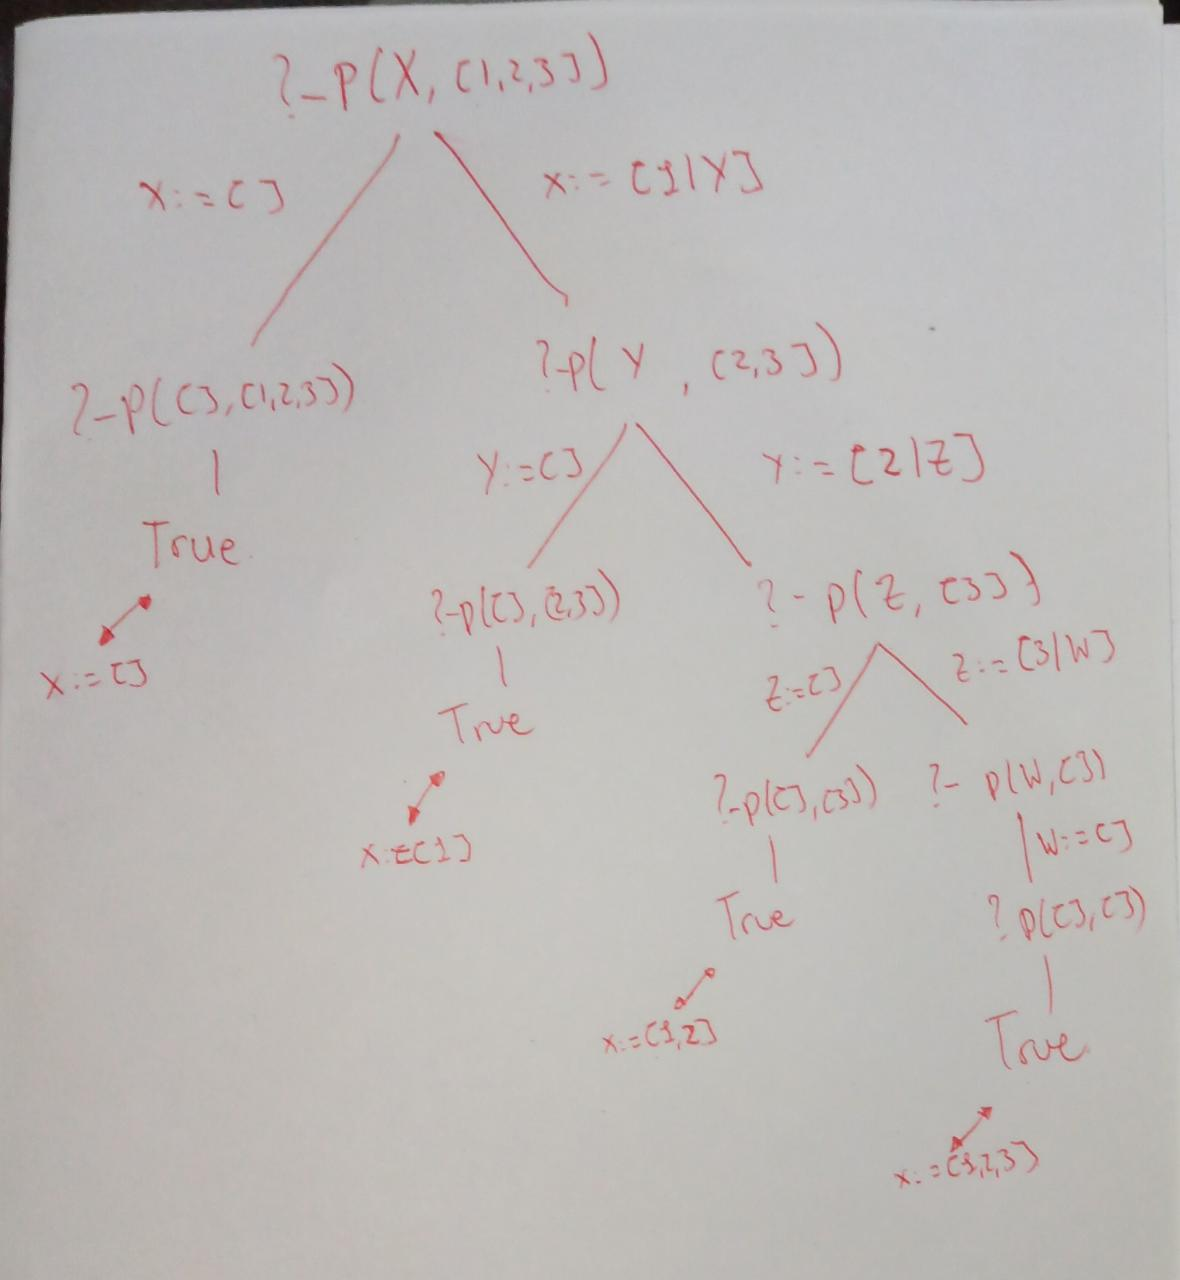
\includegraphics[scale=0.4]{9}
    \end{center}
  \end{enumerate}
\end{enumerate}


\end{document}
